\section{Auswertung}
\label{sec:Auswertung}

Die für die verschiedenen Heizströme $I_{\text{Heiz}}$ bzw. Heizspannung $U_{\text{Heiz}}$ gemessenen Werte sind in den Tabellen (\ref{tab:Kennlinie_1_2}),
(\ref{tab:Kennlinie_3_4}) und (\ref{tab:Kennlinie_5}) aufgetragen. Die verschiedenen Kennlinien sind in den Abbildungen (\ref{fig:plot_1}) und (\ref{fig:plot_2}) dargestellt. 

\begin{figure}
    \centering
    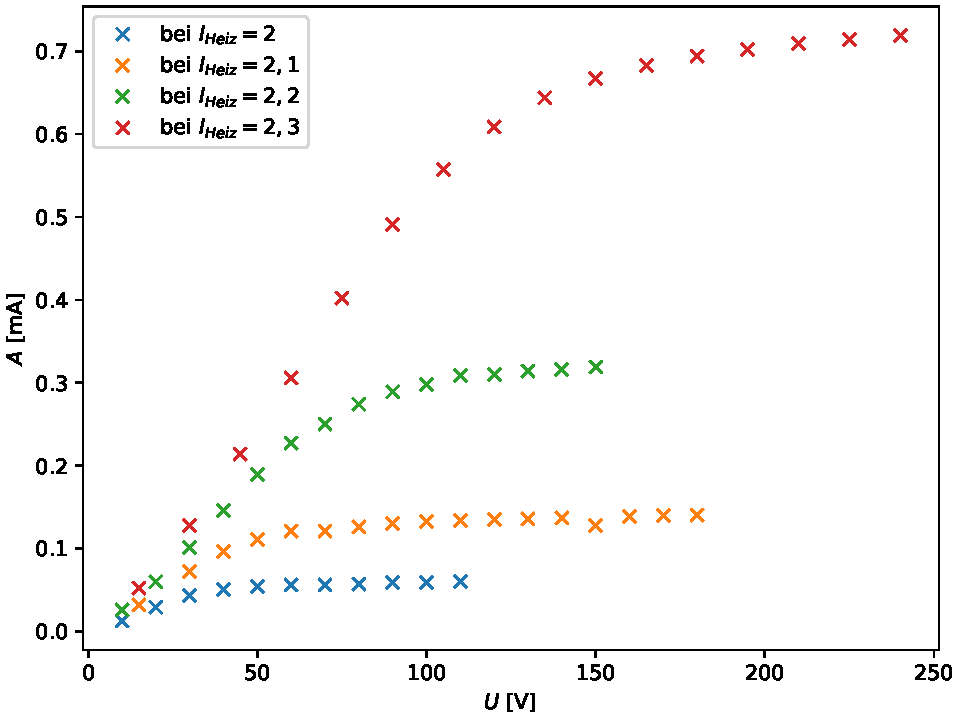
\includegraphics[width=0.8\textwidth]{plot_1.pdf}
    \caption{Kennlinien der Diode bei verschiedenen Heizströmen.}
    \label{fig:plot_1}
\end{figure}
\begin{figure}
      \centering
      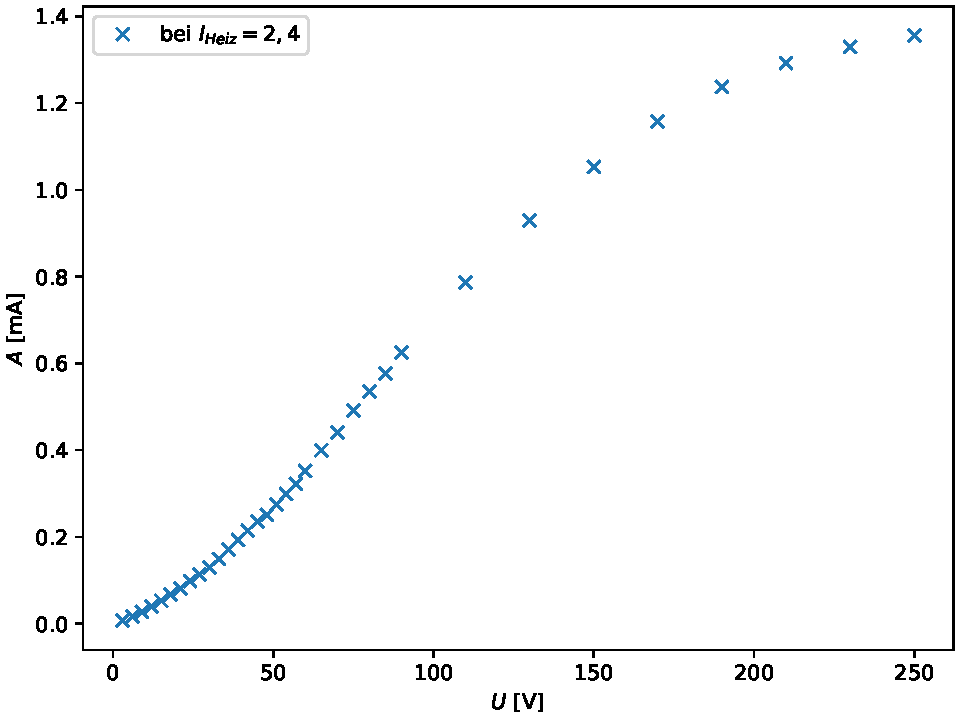
\includegraphics[width=0.8\textwidth]{plot_2.pdf}
      \caption{Kennlinien der Diode bei einem Heizstrom von 2,4 mA}
      \label{fig:plot_2}
\end{figure}

Aus den Abbildungen (\ref{fig:plot_1}) und (\ref{fig:plot_2}) werden die Sättigungsströme $I_S$ abgelesen, die in Tabelle (\ref{tab:Kennlinie_5}) aufgelistet sind.
\begin{table}[H]
    \centering
    \caption{Gemessener Sättigungstrom in Abhängigkeit vom Strom bei $I_{\text{Heiz}} = 2,4$ und $U_{\text{Heiz}} = 5$.}
    \label{tab:Kennlinie_5}
    \begin{tblr}{colspec={c c}}
        \toprule
        $I \left[\unit{\milli\ampere}\right]$ & $I_{S} \left[\unit{\milli\ampere}\right]$ \\
        \midrule  
        2,0 &  0,060 \\
        2,1 &  0,140 \\
        2,2 &  0,319 \\
        2,3 &  0,719 \\
        3,4 &  1,356 \\
        \bottomrule
    \end{tblr}
\end{table}

\subsection{Gültigkeit des Langmuir-Schottkyschen Raumladungsgesetzes}
Die Langmuir-Schottkysche Gleichung (\ref{eqn:Raumladungsgesetz}) hat die Form $I = a \cdot U^b$. Diese lässt sich durch Logarithmisieren 
in die Geradengleichung 
    \begin{equation*}
    \log(I) = b \cdot \log(U) + \log(a)
    \end{equation*}
bringen. Zur Überprüfung der Gleichung wird eine lineare Regression der 5. Kennlinie verwendet, die bei dem 
höchsten Heizstrom entsteht. Die Regression und die Messwerte der 5. Kennlinie sind in Abbildung (\ref{fig:plot_3}) abgebildet. 
\begin{figure}
    \centering
    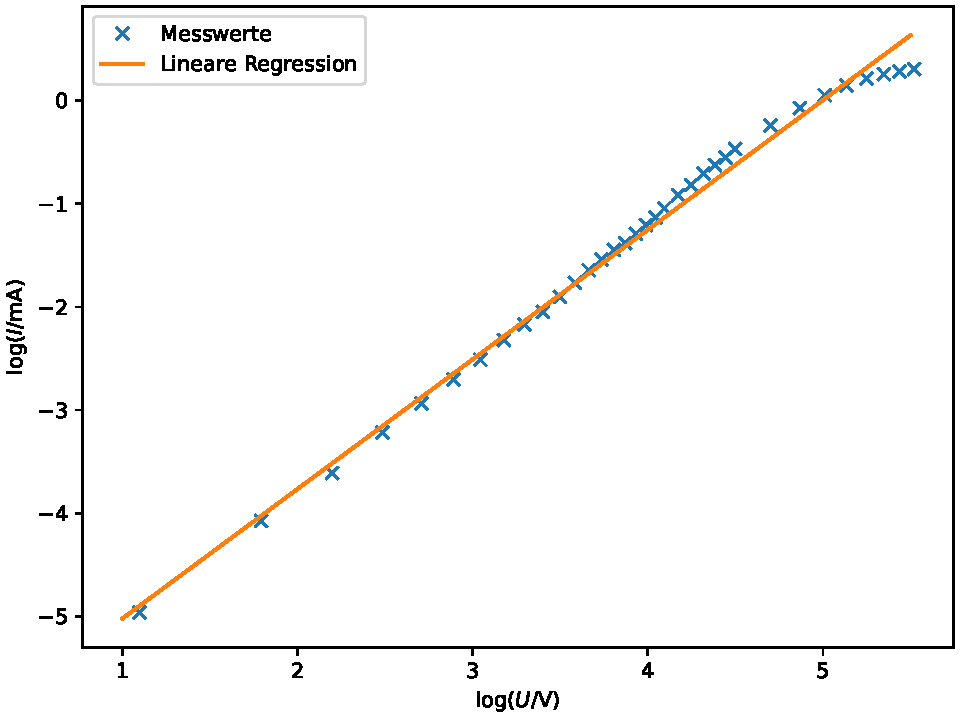
\includegraphics[width=0.8\textwidth]{plot_3.pdf}
    \caption{Lineare Regression der logarithmisierten, fünften Kennlinie.}
    \label{fig:plot_3}
\end{figure}

Durch die lineare Regression ergeben sich 
die Werte
\begin{align}
    \log(a) &= 1,26 \pm 0,02 \\
    b &= -6,28 \pm 0,08 \, .
\end{align}
$b$ ist zur Auswertung der Gültigkeit nicht relevant. $\log(a)$ kann mit dem Theoriewert $\log(a)_{\text{Theo}}= \frac{3}{2}$ verglichen werden.

\subsection{Bestimmung der Kathodentemperatur}
Der Bereich des Anlaufstroms hat einen exponentiellen Zusammenhang zwischen Strom und 
Spannung wie in Gleichung (\ref{eqn:Anlaufstrom}) zu sehen ist. Die Messwerte werden bei einem Heizstrom
von $2,3 \,\unit{\ampere}$ aufgenommen. Durch das Logarithmieren des Stroms 
und dem Auftragen gegen die Spannung kann eine lineare Regression der Form 
$$y = cx + d$$
durchgeführt werden. Die verwendeten Messwerte aus dem Anlaufbereich sind in Tabelle (\ref{tab:Anlaufbereich}) zu sehen. 

Diese Messwerte und die lineare Regression sind in Abbildung (\ref{fig:plot_3}) dargestellt. 
\begin{figure}
    \centering
    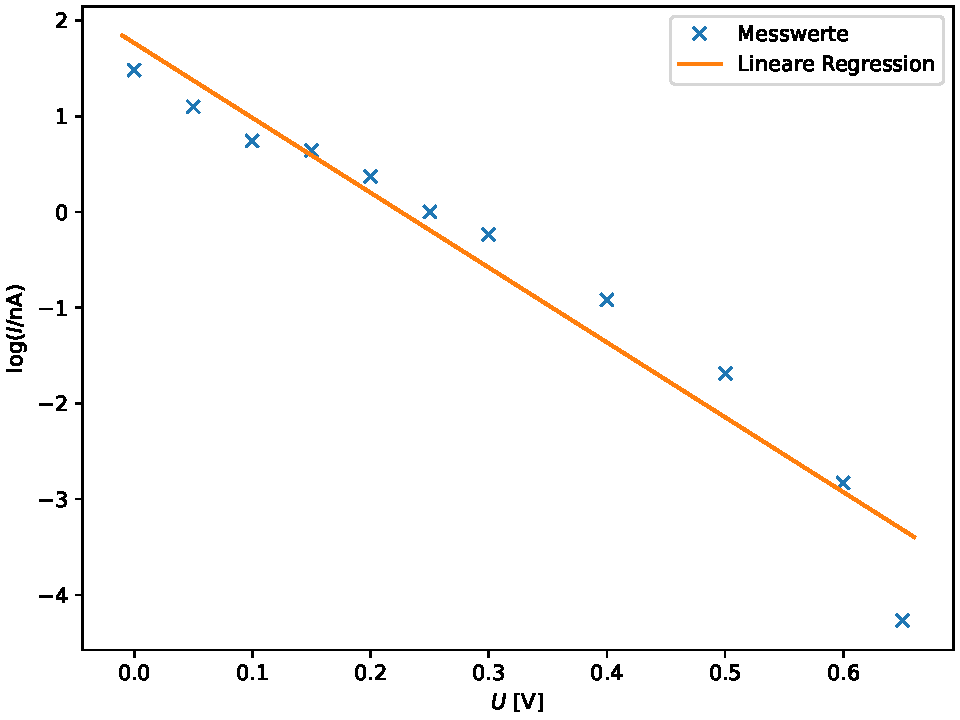
\includegraphics[width=0.8\textwidth]{plot_4.pdf}
    \caption{Lineare Regression der Messwerte aus dem Anlaufbereich.}
    \label{fig:plot_3}
\end{figure}
Die Wert der lineare Regression bestimmen sich zu 
\begin{align*}
    c &= -7,8 \pm 0,6 \\
    d &= 1,7 \pm 0,2 \, .
\end{align*}
Durch Vergleich mit Gleichung (\ref{eqn:Anlaufstrom}) ergibt sich 
\begin{align*}
    c &= -\frac{e}{kT} \\
    \Leftrightarrow T &= -\frac{e}{kc}
\end{align*}
für die Kathodentemperatur $T$. 
Die aus den Messwerten bestimmte Kathodentemperatur ist 
$$ T = (1,5 \pm 0,1)\cdot 10^{3} \, \, \unit{\kelvin}\,.$$

\subsection{Bestimmung der Kathodentemperaturen und Austrittsarbeit von Wolfram}
Zur Bestimmung der Kathodentemperatur wird Gleichung (\ref{eqn:aufWunschvonAmelie}) nach 
$$ T = \left(\frac{I_H \cdot U_H - N_{WL}}{f\eta\sigma}\right)^{1/4} $$
umgestellt. 
Für die verwendete Kathode gelten folgende Werte: Die Wärmeleistung beträgt
$W_{NL} = 0,95 \, \unit{\watt}$, die emmitierende Fläche ist $f = 0,32 \unit{\centi\meter\squared}$
und der Emissionsgrad ist $\eta = 0,28$. 
Die Ergebnisse sind in Tabelle (\ref{tab:Kathodentemperatur_experiment}) aufgeführt. 
\begin{table}[H]
    \centering
    \caption{Kathodentemperaturen in Abhängigkeit des Heizstroms und der Heizspannung.}
    \label{tab:Kathodentemperatur_experiment}
    \begin{tblr}{colspec={c c c}}
        \toprule
        $\text{Strom} \left[\unit{\milli\ampere}\right]$ & $\text{Spannung} \left[\unit{\volt}\right]$ & $\text{Temperatur} \left[\unit{\kelvin}\right]$\\
        \midrule  
            2   & 4   & 1927,53 \\
            2,1 & 4   & 1954,31 \\
            2,2 & 4,5 & 2046,02 \\
            2,3 & 5   & 2131,90 \\
            2,4 & 5   & 2131,90 \\
        \bottomrule
    \end{tblr}
\end{table}
Durch das Ersetzen von $j_S = \frac{I_S}{f}$ wird die Austrittsarbeit mithilfe von 
$$\Phi = - \frac{kT}{e} \log{\left(\frac{I_S h³}{4\pi f e m_0k²T²}\right)} $$
berechnet.
Mithilfe der in Tabelle (\ref{tab:Kathodentemperatur_experiment}) vermerkten Werte wird die 
Austrittsarbeiten berechnet, die in Tabelle (\ref{tab:Austrittsarbeit}) aufgelistet sind.
\begin{table}[H]
    \centering
    \caption{Austrittsarbeit in Abhängigkeit des Heizstroms.}
    \label{tab:Austrittsarbeit}
    \begin{tblr}{colspec={c c}}
        \toprule
        $\text{Strom} \left[\unit{\milli\ampere}\right]$ & $\Phi \left[\unit{\eV}\right]$ \\
        \midrule  
            2   & 5,12 \\
            2,1 & 5,05 \\
            2,2 & 5,16 \\
            2,3 & 5,24 \\
            2,4 & 5,19 \\
        \bottomrule
    \end{tblr}
\end{table}
Der Mittelwert dieser Werte wird zu $\bar{\Phi} = (5,15 \pm 0,03) \, \unit{\eV}$ bestimmt.


%Siehe \autoref{fig:plot}!